\chapter{Results}
\begin{comment}


\end{comment}

\section{Results from the Lenard-Jones Potential with direct Summation}
\begin{comment}

\end{comment}

% Plot of the total energy as a function of time
\begin{figure}
	\begin{center}
		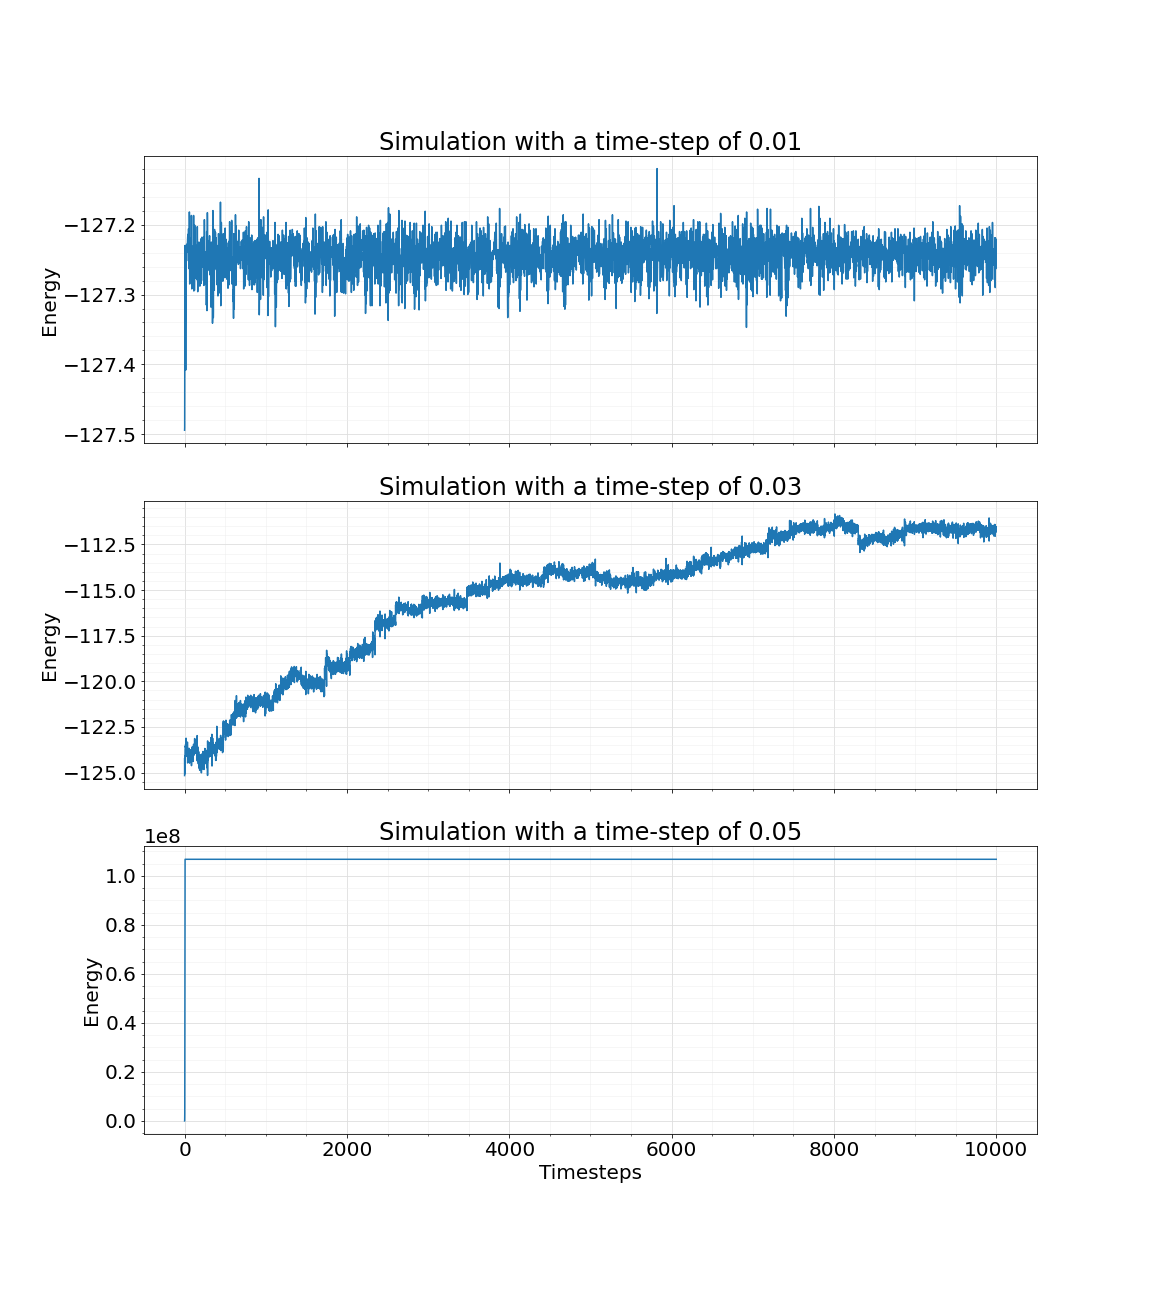
\includegraphics[scale= 1.0]{/home/cm/CLionProjects/MDCode/AData//totalEnergyDrift.png}
	\end{center}
	\caption[Simulation with different timesteps]{Simulation with different timesteps}
	\label{SimWithTimestep}
\end{figure}
The first task of the course asks to plot the total energy of the simulation for different time steps. The units were in a Lenard-Jones equivalent and not given here. As can be seen in the sequence \ref{SimWithTimestep}, as the timesteps get, the energy in the simulation goes from stable (timestep 0.01) over a drifting behavior (timestep 0.03) to being unstable (timestep 0.05). A good timestep for this simulation would be 0.01.  
\par
To visualize the simulation OVITO \cite{ovito} was used and this series of images was created.
% Simulation Snapshots
\begin{figure}
	\begin{center}
		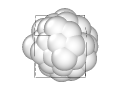
\includegraphics[scale= 0.65]{Figure/1ImageS.png}
	\end{center}
	\caption[Simulation Snapshot]{Simulation Snapshot}
	\label{SimulationSnapshot1}
\end{figure}

\begin{figure}
	\begin{center}
		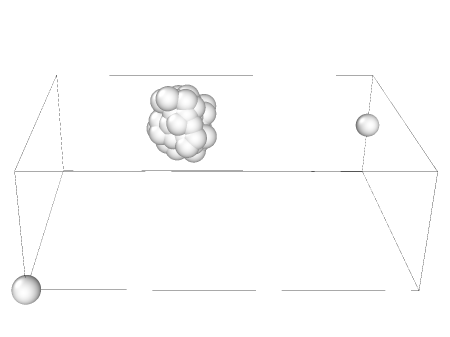
\includegraphics[scale= 0.75]{Figure/2ImageS.png}
	\end{center}
	\caption[Simulation Snapshot]{Simulation Snapshot }
	\label{SimulationSnapshot2}
\end{figure}

\begin{figure}
	\begin{center}
		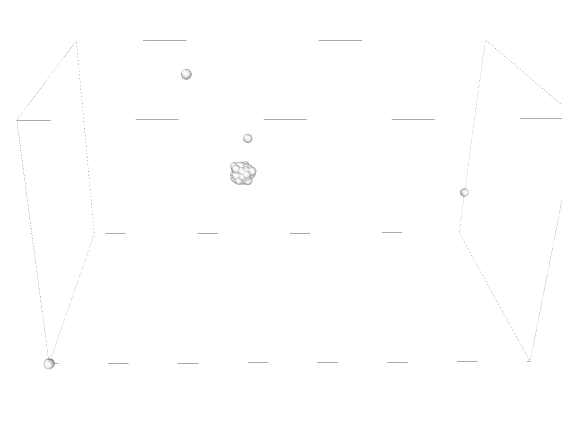
\includegraphics[scale= 0.65]{Figure/3ImageS.png}
	\end{center}
	\caption[Simulation Snapshot]{Simulation Snapshot }
	\label{SimulationSnapshot3}
\end{figure}
As it can be seen in the images \ref{SimulationSnapshot1}, \ref{SimulationSnapshot2} and \ref{SimulationSnapshot3} the Atoms are initially ordered into a blob, which was given in the course. 
Later in the simulation some of the atoms escaped the initial blob and flew outward separately. 
\section{Result from the Simulation with the Berendsen Thermostat}
\begin{comment}
computational complexity 
why on2
optimization not every force is looked at individually as the force resluting form this atom is the same for the other atom but negative
\end{comment}
After incorporating the Berendsen Thermostat into the code it is interesting to look at the computational complexity of the simulation. With growing numbers of atoms the computation of should follow an order of something like O(N²). The main culprit for this is the force-computation, as each interaction with all the other atoms in the simulation has to be computed. This is also shown in the next figure as the computation time seems to follow a quadratic function. 
\begin{figure}
	\begin{center}
		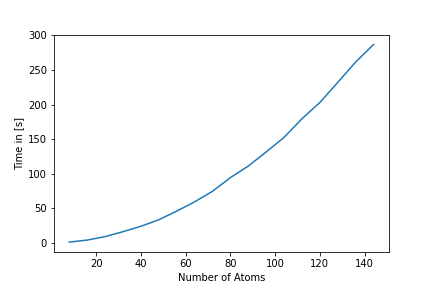
\includegraphics[scale=1]{Figure/plotAtomTimes.png}
	\end{center}
	\caption[Simulationtime with the Berendsen Thermostat from 8 to 192 Atoms]{Simulationtime with the Berendsen Thermostat from 8 to 192 Atoms }
	\label{PlotSimulationTimeBerendsenThermostat}
\end{figure}
Although all the interaction between all the atoms are computed the individual forces do not carry the same weight to the force that affects the atom. It should be rather clear that, the further apart atoms are, the smaller the forces get. After a certain distance it gets so small that it can be ignored. This leads to the idea to use neighborhood-lists that ignore the atoms outside of a certain radius, which was done in the next section.

\section{Results from the Simulation with the Neighborhood-List}
\begin{comment}

\end{comment}
After running the simulation in the previous section, it was clear that they follow a computational complexity of the order O(N²). This can be reduced to a linear order O(N) with the usage of neighborhood-lists. Only the atoms in a certain radius around the atom will be considered and a force will be added to the total force affecting the atom. This can be seen in figure \ref{PlotSimulationTimesCutoffNew} on a linear and a logarithmic scale.  
\begin{figure}
	\begin{center}
		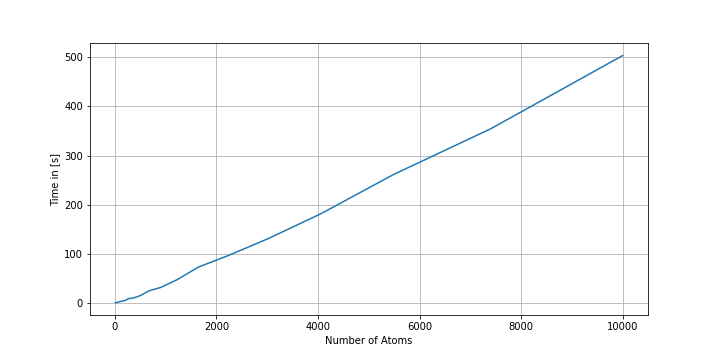
\includegraphics[scale=1.25]{Figure/plotAtomTimesMoreData.png}
	\end{center}
	\caption[Simulationtime with the Neighborhood-List]{Simulationtime with the Neighborhood-List}
	\label{PlotSimulationTimesCutoffNew}
\end{figure}

\section{Results from the Simulation with the Embedded-Atom Method Potential}
\begin{comment}
1 graph
- potential energy gets less with an increase to the clustersize
- the 

2 
Heat capacity and latent heat should converge
\end{comment}
In the next step the Embedded-Atom Method Potential was used to compute the potential energy and the forces between the atoms. A neighborhood-list was also used. With this it is possible to look at the actual physical properties of the materials - in this case gold. In figure \ref{GoldClusterSimulationTemperaturEnergy4In1} energy and temperature for different cluster sizes are plotted. It is possible to extract the melting point, the heat-capacity and the latent-heat from this diagram. This can be seen in the next figure \ref{GoldClusterSimulationVsClustersize} in relation to the size of the atom-cluster. All data in this figure has been read by hand so it has to be taken with a grain of salt. 

\par 
The first interesting property is the melting point of the cluster, which can be seen in the different curvature in the graphs in figure \ref{GoldClusterSimulationTemperaturEnergy4In1} (for the red graph at 900K for example). The melting point increases as the clusters get bigger, but is still not not near it's macroscopic equivalent of 1337 K. 

\par
It can also be seen that the potential energy of the median atom decreases with bigger clustersizes. To explain this, the ratio of surface to volume of the cluster and the fact that atoms at the border of the cluster need to have a higher energy, have to be considered. With increased clustersizes a smaller percentage of atoms is at the edge which leadsto an increases in the total energy of the cluster. 
The slope of the curvature at the melting point also increases with bigger clustersizes. In a big physical system this would be a straight line where the actual melting point is and the simulated system seems to converge to that. 

\begin{figure}
	\begin{center} 
		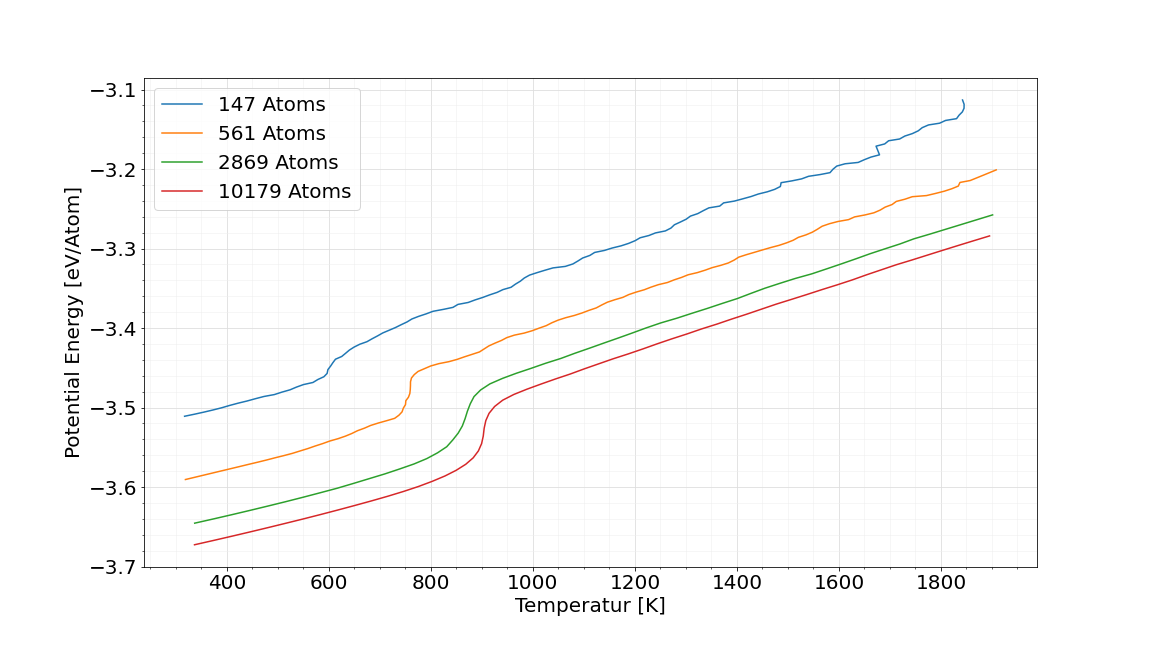
\includegraphics[scale=1.15]{/home/cm/CLionProjects/MDCode/AData/Clusters/temperaturPotentialEnergyCurveMoreInOne.png} 
	\end{center} 
	\caption[Gold Cluster Simulation]{Gold Cluster Simulation} 
	\label{GoldClusterSimulationTemperaturEnergy4In1} 
\end{figure} 

In the diagram of figure \ref{GoldClusterSimulationVsClustersize} which plot the heat capacity and the latent heat, it can be seen that both seem to converge. The melting point on the other hand still seems to increase as it is still away from it's true melting point.

\begin{figure}
	\begin{center} 
		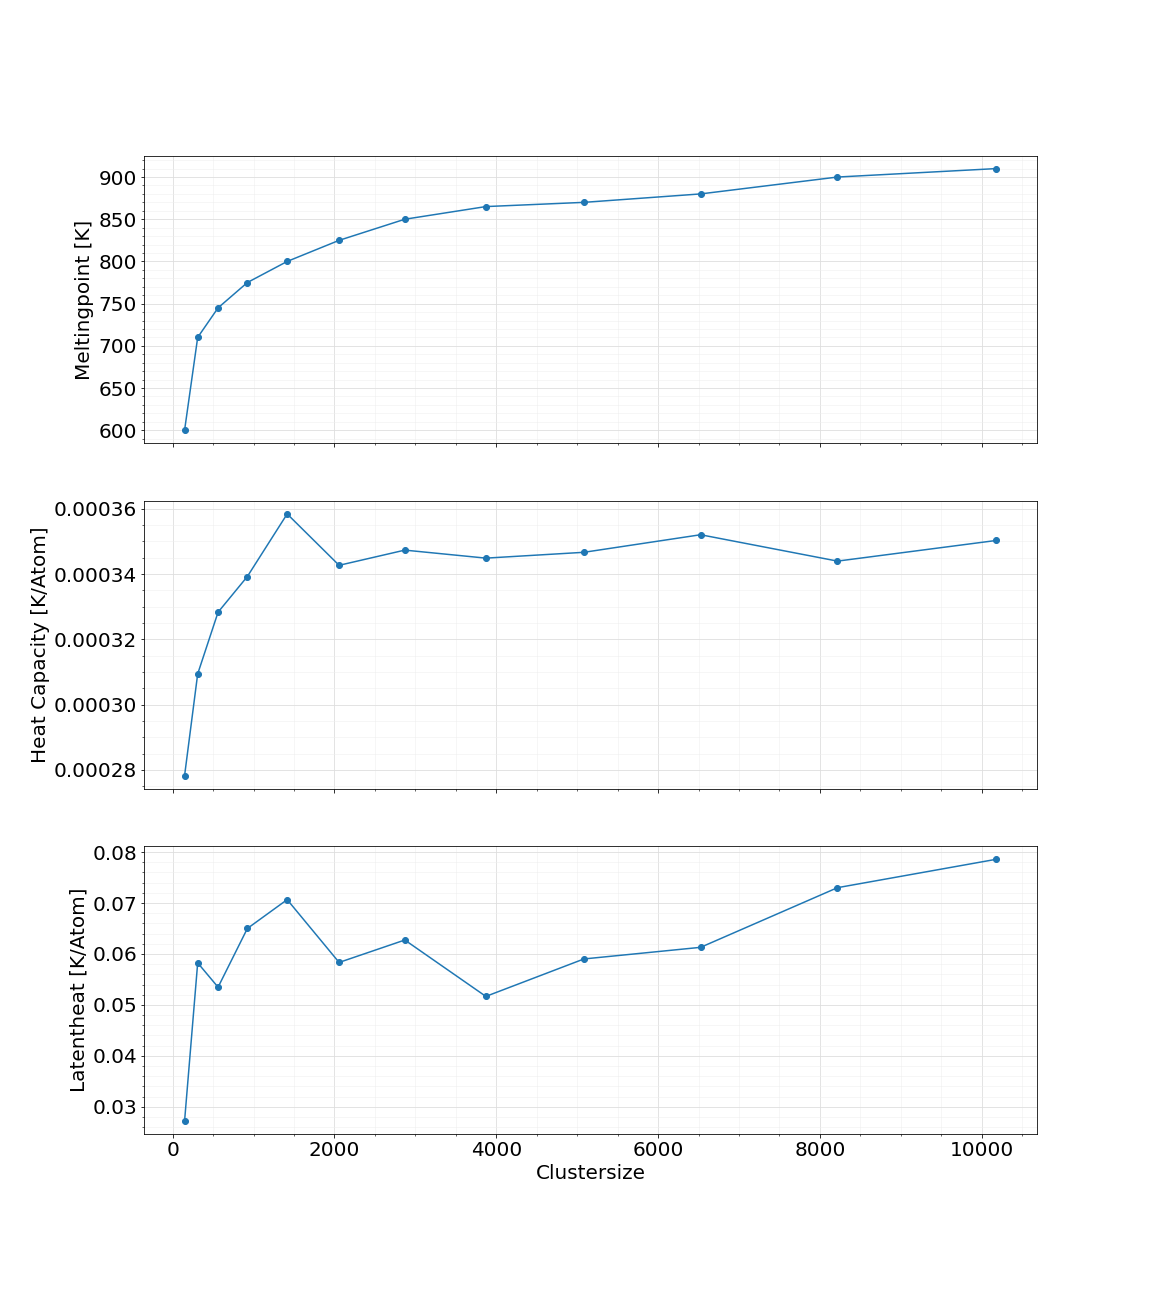
\includegraphics[scale=1.15]{/home/cm/CLionProjects/MDCode/AData/Clusters/VsClusterSizeAll.png} 
	\end{center} 
	\caption[Melting Point, Heat Capacity and Latent Heat vs Clustersize]{Melting Point, Heat Capacity and Latent Heat vs Clustersize} 
	\label{GoldClusterSimulationVsClustersize} 
\end{figure} 
